\begin{ledgroupsized}[r]{120mm}
\footnotesize 
\pstart 
\noindent\textbf{\"{U}berlieferung:}
\pend
\end{ledgroupsized}
\begin{ledgroupsized}[r]{114mm}
\footnotesize 
\pstart \parindent -6mm
\makebox[6mm][l]{\textit{L}}Auszüge mit Bemerkungen aus R. \textsc{Hooke},\cite{00332} \title{Animadversions on the First Part of the Machina Coelestis of Johannes Hevelius}, London 1674: LH XXXV 15, 6 Bl. 9-16. 4 Bog. 4\textsuperscript{o}. 13 \nicefrac{1}{2} S. Bl. 9 leer. Der Text beginnt auf Bl. 10~r\textsuperscript{o}. Bl. 9 und Bl. 16 bilden einen Bogen, der die weiteren drei Bogen (Bl. 10-11, 12-13, 14-15) umfasst. Zeichnungen mit umlaufendem Text sowie leer gelassene Stellen, an denen die von Leibniz besprochenen Figuren hier aus der Vorlage erg\"{a}nzt werden. Zwei Wasserzeichen.\\ Cc 2, Nr. 921 \pend
\end{ledgroupsized}

\vspace*{5mm}
\begin{ledgroup}
\footnotesize 
\pstart
\noindent\footnotesize{\textbf{Datierungsgr\"{u}nde}: Hookes \textit{Animadversions} erschienen 1674 in London. Oldenburg erw\"{a}hnt eine Schrift dieses Inhalts in seinem Brief an Leibniz vom 8. (18.) Dezember 1674 (\textit{LSB} III, 1 N. 41). Kurz danach werden Hookes \textit{Animadversions} in den \textit{Philosophical Transactions} 9 (1674), S. 215f.\cite{00158} besprochen. Schlie{\ss}lich teilt Leibniz Oldenburg am 30. M\"{a}rz 1675 mit: \textit{Vidi Hookianam diatriben de apparatu Heveliano} (\textit{LSB} III, 1 N. 46.3). Die Wasserzeichen sind für die Zeit von Frühjahr bis Dezember 1675 belegt.}
\pend
\end{ledgroup}
\count\Afootins=1200
\count\Bfootins=1200
\count\Cfootins=1200
\vspace*{8mm}
\pstart 
\normalsize\noindent
[10~r\textsuperscript{o}]
\textit{Animadversions on the first part of the Machina coelestis, of the Honourable learned and deservedly famous Astronomer Johannes Hevelius\cite{00329}}\protect\index{Namensregister}{\textso{Hevelius}, Johannes (1611-1687)} \textit{consul of Dantzigk}\protect\index{Ortsregister}{Danzig} \textit{together with an explication of some Instruments made by Robert} \edtext{\textit{Hooke}\protect\index{Namensregister}{\textso{Hooke}, Robert (1635-1703)}}{\lemma{\textit{Hooke}}\Cfootnote{\textsc{R. Hooke}, \textit{Animadversions}, London 1674.}} \textit{professor of Geometry in Gresham college and fellow of the Royal Society.} London\protect\index{Ortsregister}{London} printed by T. R. for John Martin\protect\index{Namensregister}{\textso{Martin}, John (?-1680)} at the bell 1674. 
\pend 
\pstart Titulus libri Heveliani: \textit{Joh. Hevelii}\protect\index{Namensregister}{\textso{Hevelius}, Johannes (1611-1687)}\textit{ Machina coelestis, pars prior organographiam sive instrumentorum Astronomicorum omnium, quibus autor hactenus sidera rimatus et dimensus est accuratam delineationem ac descriptionem plurimis iconibus aeri incisis illustratam et exornatam exhibens.}\edtext{}{\lemma{\textit{exhibens}.}\Cfootnote{a.a.O., S. 1.}}\cite{00329} Excellens ille vir insigni circumspectione, studio sumtibus, omnium Astronomorum laudes meruit. Sed si secutus fuisset methodum quam ei communicaveram, decima laboris et sumtuum parte, decies exactiorem Catalogum dedisset. Potuit correxisse quosdam errores qui in Tychonicis irrepsere; sed instrumenta ejus non sunt majoris exactitudinis capacia, quam Tychonica, etsi forte grandiora. Instrumenta Tychonis\protect\index{Namensregister}{\textso{Brahe}, Tycho 1546-1601}\protect\index{Sachverzeichnis}{instrumenta Tychonis} non minus grandia, visus utrobique nudus; divisio Heveliana\protect\index{Sachverzeichnis}{divisio Heveliana} ingeniosa, sed forte in praxi non melior, \edtext{si}{\lemma{melior,}\Bfootnote{\textit{(1)}\ imo \textit{(2)}\ si \textit{L}}} modo aequalis, Tychonicae. Tycho\protect\index{Namensregister}{\textso{Brahe}, Tycho 1546-1601} \textit{lib. 2. obs. de} \edtext{\textit{Cometa\protect\index{Sachverzeichnis}{cometa} 1577}\cite{00327}}{\lemma{\textit{Cometa 1577}}\Cfootnote{\textsc{T. Brahe}, \textit{Liber secundus de cometa anni 1577}, Prag 1603, S. 461\cite{00327} (\textit{TBO} IV, S. 372.)}} divisionem graduum in singula minuta (: per lineas diagonales, et horum in dena scrupula secunda subdivisionem [:)], in omnibus se machinis Astronomicis usurpare; licet enim ejus demonstratio sit tantum in rectilineis Geometrice exacta, tamen arcualibus in \edtext{tam exili}{\lemma{tam}\Bfootnote{\textit{(1)}\ exiguo \textit{(2)}\ exili \textit{L}}} interstitio, quod a recta linea insensibiliter differt tuto applicari. Altera, inquit idem Tycho\protect\index{Namensregister}{\textso{Brahe}, Tycho 1546-1601} divisio\protect\index{Sachverzeichnis}{divisio Nonnii} imitatione \textit{Petri Nonnii}\protect\index{Namensregister}{\textso{Nu\~{n}ez}, Pedro (1502-1578)}\textit{, qui eam proposuit libro de Crepusculis\cite{00328}} \edtext{\textit{prop. 3.}}{\lemma{\textit{prop. 3}.}\Cfootnote{\textsc{P. Nu\~{n}ez}, \textit{De Crepusculis}, editio 2\textsuperscript{da}. Coimbra 1571, S. 20f.\cite{00328}}} \textit{per plures quadrantis\protect\index{Sachverzeichnis}{quadrans} arcus introrsum descriptos, et diversimode} \edtext{\textit{subdivisos.} Addit}{\lemma{\textit{subdivisos}}\Bfootnote{\textit{(1)}\ \textit{, ait} \textit{(2)}\ . Addit \textit{L}}}\edtext{}{\lemma{\textit{subdivisos}.}\Cfootnote{\textsc{R. Hooke}, \textit{Animadversions}, S. 3.}} ei aliquid a se auctarii loco \textit{additum esse, ita ut exterior arcus in plurimas portiunculas dividatur, neque is ordo aut numerus arcuum sese introrsum comitantium, quem ille praefinivit, sed multo expeditior et perfectior observetur}\edtext{}{\lemma{\textit{observetur}}\Cfootnote{a.a.O., S. 3f.}} (: addit Hookius\protect\index{Namensregister}{\textso{Hooke}, Robert (1635-1703)} videri eandem esse quam nunc adhibuit Hevelius\protect\index{Namensregister}{\textso{Hevelius}, Johannes (1611-1687)} :) tamen quod sit plus in ea laboris quam fructus in usu apud se esse desiisse. Adde quae dicit lib. 1. de stella nova 1572.
\edtext{pag. 671.}{\lemma{pag. 671.}\Cfootnote{\textsc{T. Brahe}, \textit{Astronomiae instauratae progymnasmata}, Prag 1602, S. 671 (\textit{TBO} III, S. 184f.).}}\cite{01119}
The \textit{way of diagonals first made use of in }\textit{England}\protect\index{Ortsregister}{England} \textit{by the most skilful mathematician Richard
\edtext{Cantz\-ler\protect\index{Namensregister}{\textso{Cantzler}, Richard}}{\lemma{\textit{Cantzler}}\Cfootnote{\textsc{R. Hooke}, \textit{Animadversions}, S.~4.}}}
%\textit{by the most skilful mathematician Richard Cantz\-ler}\protect\index{Namensregister}{\textso{Cantzler}, Richard (??)}\edtext{}{\lemma{\textit{mathematician}}\Cfootnote{\textsc{R. Hooke}, \textit{Animadversions}, S. 4.}}
 \edtext{pag. 13 dicit Hookius\protect\index{Namensregister}{\textso{Hooke}, Robert (1635-1703)} ipsum Tychonem\protect\index{Namensregister}{\textso{Brahe}, Tycho 1546-1601} Canzlero\protect\index{Namensregister}{\textso{},} \edtext{tribuere}{\lemma{tribuere}\Cfootnote{a.a.O., 13.}}}{\lemma{}\Bfootnote{pag. [...] tribuere \textit{ erg. L}}} (+ ambigue hoc, vel
 \edtext{enim sensus:}{\lemma{enim}\Bfootnote{\textit{(1)}\ sic: \textit{(2)}\ sensus: \textit{L}}} %   enim \edtext{sensus:}{\lemma{enim}\Bfootnote{\textit{(1)}\ sic: \textit{(2)}\ sensus: \textit{L}}}
  prius in Anglia\protect\index{Ortsregister}{England} adhibitum quam alibi, inventore Canzlero\protect\index{Namensregister}{\textso{},}; vel Canzlerum\protect\index{Namensregister}{\textso{},} primum in Anglia\protect\index{Ortsregister}{England} adhibuisse; quamvis alii prius alibi: videtur affectasse hanc ambiguitatem +). Omnia Hevelii\protect\index{Namensregister}{\textso{Hevelius}, Johannes (1611-1687)} instrumenta\protect\index{Sachverzeichnis}{instrumentum Hevelii} utcunque magna virtute aequalia radio metallico tripedali cum dioptricis Tychonicis et divisione diagonalium\protect\index{Sachverzeichnis}{divisio diagonalium} quia visus nudi potentia limitata est. De quo infra. Scripseram aliquid de ea re \edtext{Hevelio\protect\index{Namensregister}{\textso{Hevelius}, Johannes (1611-1687)} 1665.}{\lemma{Hevelio 1665.}\Cfootnote{Briefwechsel zwischen Hooke und Hevelius, vgl. a.a.O., S. 5.}} Respondit in Epistola ad Soc. Regiam\protect\index{Sachverzeichnis}{Royal Society} Hevelius\protect\index{Namensregister}{\textso{Hevelius}, Johannes (1611-1687)}, telescopia\protect\index{Sachverzeichnis}{telescopium} non posse \textit{firmiter satis affigi, ut loco haud dimoveantur, etsi omnia diligentia juxta methodum descriptam per totum horizontem sint semel collocata.}\edtext{}{\lemma{\textit{collocata}.}\Cfootnote{a.a.O., S. 5.}} Ita ut dubitem usui esse posse circa restitutionem fixarum planetarumque, in majoribus distantiis capiendis; in minoribus inquit \textit{largior posse aliquid praestari. Sed an instrumenta unius spithamae radio instructa elaborari possint multo exactius quam optima quaevis vulgares dioptras\protect\index{Sachverzeichnis}{dioptra} habentia, licet 60 pedum radio elaborata, nollem adhuc} \edtext{\textit{asseverare;}}{\lemma{\textit{asseverare};}\Cfootnote{a.a.O., S. 6.}} multa in praxi non succedunt, quae in theoria videntur verissima. Si quis mihi \textit{certas observationes quarundam distantiarum et quidem fixarum circa eclipticam\protect\index{Sachverzeichnis}{ecliptica} et aequatorem existentium instrumentis, dioptricis telescopicis\protect\index{Sachverzeichnis}{telescopium} instructis; habitas} \edtext{\textit{exhiberet.}}{\lemma{\textit{exhiberet}.}\Cfootnote{a.a.O., S. 6.}} Impossibile est inquit Hookius\protect\index{Namensregister}{\textso{Hooke}, Robert (1635-1703)}, nudo visu discernere in coelis distantiam dimidio minuto primo minorem; et ex 100 vix unus distinguere potest minutum. Cumque in radio tripedali per diagonales satis habeantur dimidia minuta, sequitur omnia caetera esse inutilia. Quis est qui nudo visu discernere possit maculam lunarem Telescopicam, et sunt tamen aliquae minutum in diametro habentes et supra, v. g. Mons Sinai\protect\index{Ortsregister}{Sinai} lucida macula, in campo nigro circiter duorum minutorum diametri oculo nudo. 
%\begin{wrapfigure}{l}{0.5\textwidth}   
%\noindent                 
%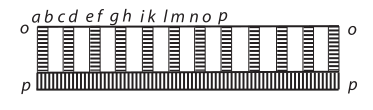
\includegraphics[trim = 0mm -3mm -5mm 0mm, clip, width=0.5\textwidth]{images/lh0351502_10r-d1.pdf}\\
%\rule[0pt]{13mm}{0mm}[\textit{Fig. 1, nach Hooke Fig. 28}]
%\end{wrapfigure}
Palus Mareotis\protect\index{Sachverzeichnis}{Palus Mareotis}, aut Lacus niger\protect\index{Sachverzeichnis}{Lacus Niger}, duae nigrae maculae in campo lucido, sunt plus quam minuti. Experimentum quod probat vim oculi limitatam, sume folium chartae albae duc in longitudinem duas parallelas oo, pp. distantia 4 aut 5 pollicum. Duc plures alias rectas ad has perpendiculares per puncta ipsius oo, transeuntes nempe per \textit{a. b. c. d. e. f. g. h. i. k. l. m. n.} \edtext{\textit{o.}}{\lemma{}\Bfootnote{\textit{o. erg. L}}} \textit{p.} distantia pollicis una ab altera. Spatia intercepta sint alternatim alba et nigra: affige parieti in radiis solis, et recede ad distantiam circiter 287 \rule[-4mm]{0mm}{10mm}$\displaystyle\frac{1}{3}$ pedum, plus minusve, ut quousque discernere potes. Ut autem distinguere possit, necesse est ut possit numerare. Haec distantia dabit virtutem oculi cujusque, unde judicari potest quantus angulus videri possit nudo visu, distincte. Altitudines solis sumi possunt ad secundi minuti exactitudinem, communi visu, si instrumentum satis largum; Nam imago solis transmissa per foramen rotundum ope superioris dioptrae\protect\index{Sachverzeichnis}{dioptra}, est repraesentata intra circulum upon the lower sight; et ope oculorum huic dioptrae\protect\index{Sachverzeichnis}{dioptra} appropinquantium, fieri potest per instrumenta satis magna, ut ad exactitudinem secundi minuti perveniatur. \edtext{Item [quodam] modo}{\lemma{Item}\Bfootnote{\textit{(1)}\ quomad \textit{(2)}\ \textbar\ quomam \textit{ \"{a}ndert Hrsg.} \textbar\ modo \textit{L}}} et in luna, cum est valde clara \edtext{quod in aliis corporibus coelestibus nemo fecit. Sed et haec via}{\lemma{clara}\Bfootnote{\textit{(1)}\ sed etiam haec ipsa via a \textit{(2)}\ quod [...] via \textit{L}}} telescopiis\protect\index{Sachverzeichnis}{telescopium} melius fieri potest, solo radii tripedalis instrumento quod fieri curavi, faciam observationes decies\\
\pend
\setline{26}
\vspace{0.5em}
\pstart
\begin{center}  
   \hspace{13mm} 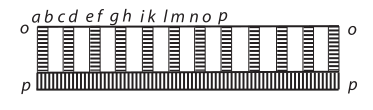
\includegraphics[trim = 0mm 5mm 0mm 0mm, clip, width=0.55\textwidth]{images/lh0351502_10r-d1.pdf}
\newline
\centering
[\textit{Fig. 1, nach Hooke Fig. 28}]
\end{center}  
\pend
\newpage
\pstart \noindent accuratiores; exceptis solaribus \edtext{quam maximis Hevelianis}{\lemma{}\Bfootnote{quam maximis Hevelianis \textit{erg. L}}} quanta ad pinnacidia quadrantis\protect\index{Sachverzeichnis}{quadrans} aenei Heveliani de quibus \edtext{pag. 98.}{\lemma{pag. 98.}\Cfootnote{\textsc{J. Hevelius}, \textit{Machinae Coelestis Pars Prior}, Danzig 1673, S. 98.\cite{00329}}} ille pro altitudine solis sumenda, haec bene quidem; sed \edtext{meliora adhibito}{\lemma{}\Bfootnote{meliora \textbar\ si \textit{gestr.}\ \textbar\ adhibito \textit{L}}} vitro objectivo, etiam sine Tubo. Ita semi quam voluisset \edtext{dedisset magnitudinem superiori dioptrae\protect\index{Sachverzeichnis}{dioptra} et imagini solis}{\lemma{dedisset}\Bfootnote{\textit{(1)}\ claritatem radiis solis \textit{(2)}\ magnitudinem [...] solis \textit{L}}}, idque sine specie penumbrae\protect\index{Sachverzeichnis}{penumbra}, posito inferiorem dioptram\protect\index{Sachverzeichnis}{dioptra} debita distantia vitri objectivi. Divisio Tychonica\protect\index{Sachverzeichnis}{divisio Tychonica} hodie vulgo nota, per diagonales, quae parallelos circulos secant, hanc ipse Tycho\protect\index{Namensregister}{\textso{Brahe}, Tycho 1546-1601} tribuit Anglico Mathematico Canzlero\protect\index{Namensregister}{\textso{},}. Observavit Hevelius\protect\index{Namensregister}{\textso{Hevelius}, Johannes (1611-1687)} instrumenta ex parte lignea, tamen subjecta esse errori; itaque fieri curavit ex metallo solido; ait tamen Hookius\protect\index{Namensregister}{\textso{Hooke}, Robert (1635-1703)} Christophorum Wrennum\protect\index{Namensregister}{\textso{Wren}, Christopher (1632-1723)} fecisse satis bona, modo laminae divisiones recipientes ex metallo. Caeterum ex instrumentis Hevelius\protect\index{Namensregister}{\textso{Hevelius}, Johannes (1611-1687)} recipit tantum sextantes\protect\index{Sachverzeichnis}{sextans}, Quadrantes\protect\index{Sachverzeichnis}{quadrans}, Octantes, rejectis: Radiis, Astrolabiis, Zodiacalibus vel Aequinoctialibus annulis, parallacticalibus instrumentis or Hoops nos tamen inquit Hook\protect\index{Namensregister}{\textso{Hooke}, Robert (1635-1703)} infra ostendemus, quosdam ex iis esse necessarios. Methodum subdividendi quadrantem\protect\index{Sachverzeichnis}{quadrans} ab Hedraeo\protect\index{Namensregister}{\textso{Hedraeus}, Bengt (1608-1659)} in praxin traductam magni facit Hevelius\protect\index{Namensregister}{\textso{Hevelius}, Johannes (1611-1687)}. Benedictus Hedraeus\protect\index{Namensregister}{\textso{Hedraeus}, Bengt (1608-1659)} 1643\cite{00330} \edtext{librum}{\lemma{librum}\Cfootnote{\textsc{B. Hedraeus}, \textit{Nova et accurata astrolabii geometrici structura}, Leiden 1643.\cite{00330}}} edidit circa novam et accuratam [10~v\textsuperscript{o}] structuram Astrolabii Geometrici.
\pend 